% !TeX root = ../main-english.tex
% !TeX spellcheck = en-US
% !TeX encoding = utf8
% -*- coding:utf-8 mod:LaTeX -*-

%This smart spell only works if no changes have been made to the chapter
%using the options proposed in preambel/chapterheads.tex.
\setchapterpreamble[u]{%
	\dictum[Albert Einstein]{We cannot solve our problems with the same level of thinking that created them}
}
\chapter{Introduction}
\label{chap:k1}

Look mom, some text!

\section{Brain state spaces}
This is an introduction into brain states and functional alignment
\pagebreak

\section{Magnetoencephalograpy (MEG)}
This is an introduction into \gls{meg} data
\pagebreak

\section{Research data management for computational modeling}
%This is an introduction on the importance of research data management for reproducible science

Research data encompasses everything that is produced in the life span of a research project.
It could include raw data acquisitions, preprocessed or otherwise standardized datasets, software, analysis scripts, results, compiled reports or articles, figures, tables, interviews - and many other final or intermediate outcomes of a research process.
\gls{rdm} describes the handling of this research data through its entire life cycle: from curation, use, publication and sharing, archiving to re-use or destruction.
Typically, research data have a much longer life span than the project that creates them.
Increasing reusability

The field of neuroimaging is characterized by complex datasets, typically encompassing different modalities (such as imaging, electro-physiological, and behavioral measurements), and multi-stepped, often exploratory analysis workflows \citep{poline2011}.
% add more on RDM

Additionally, the growing awareness of the role of sample size for robust results \citep{button2013power} \citep{turner2018small} and a focus on diverse, representative samples has resulted in datasets of unprecedented size.
In the neurosciences, datasets scale to millions of files, hundreds of terabytes6,7, acquired from tens of thousands of participants. Well known examples, such as the Human Connectome Project8, the Adolescent Brain Cognitive Development Study (ABCD)9, or the UK Biobank (UKB) project10, contain diverse data ranging from brain imaging to genetics to clinical and non-clinical measures.

This chapter will further showcase how research data management is a foundational element of reproducible research.



The following section will highlight one of several software tools that aids with the complex tool of research data management: DataLad. The following \cref{chap:k1} will outline how software usability can improve scientific practice, using DataLad and its user-facing documentation, the DataLad Handbook, as an example.
The upcoming \cref{chap:k2} will then focus specifically on two aspects of research data management for reproducibility: Software environments, and scalability to large sample sizes.


% What is research data management
%% FAIR
\gls{rdm}
% Why is it important
%% Reproducibility crisis


% What can we do to improve research data management
%% BIDS, read Niso paper

The building blocks of scientific results extend to more than the files that constitute the actual research output, but also to all elements involved in its generation \citep{claerbout1992electronic}.
Consider three types of research output: Raw data originates from acquisitions based on - potentially ongoing - experiments, raw data transformations, or data cleaning, processed data or results stem from computations with analysis code or software in specific versions on particular data, and software, expressed in raw (code) or derived (transformed into executable) form, is created or used in specific computational environments, with compilers, underlying libraries, and systems in distinct versions.
Those building blocks are integral information to retrace the genesis, reproduce, or trust research outputs (Kennedy et al., 2019), but they are rarely ever static.
Whatever created a given output evolves during usually incremental processes such as continuous quality control, acquisition, maintenance, or project revision.
However, changes in these building blocks will influence the resulting research output \citep{kennedy2019everything} 2019),\citep{glatard2015reproducibility}.
If it is not possible to precisely identify the foundational elements and everything involved in their creation, the reproducibility and reusability of research outputs and projects that use these objects is hence threatened \citep{kennedy2019everything}.

% provenance
\begin{figure}
	\centering
	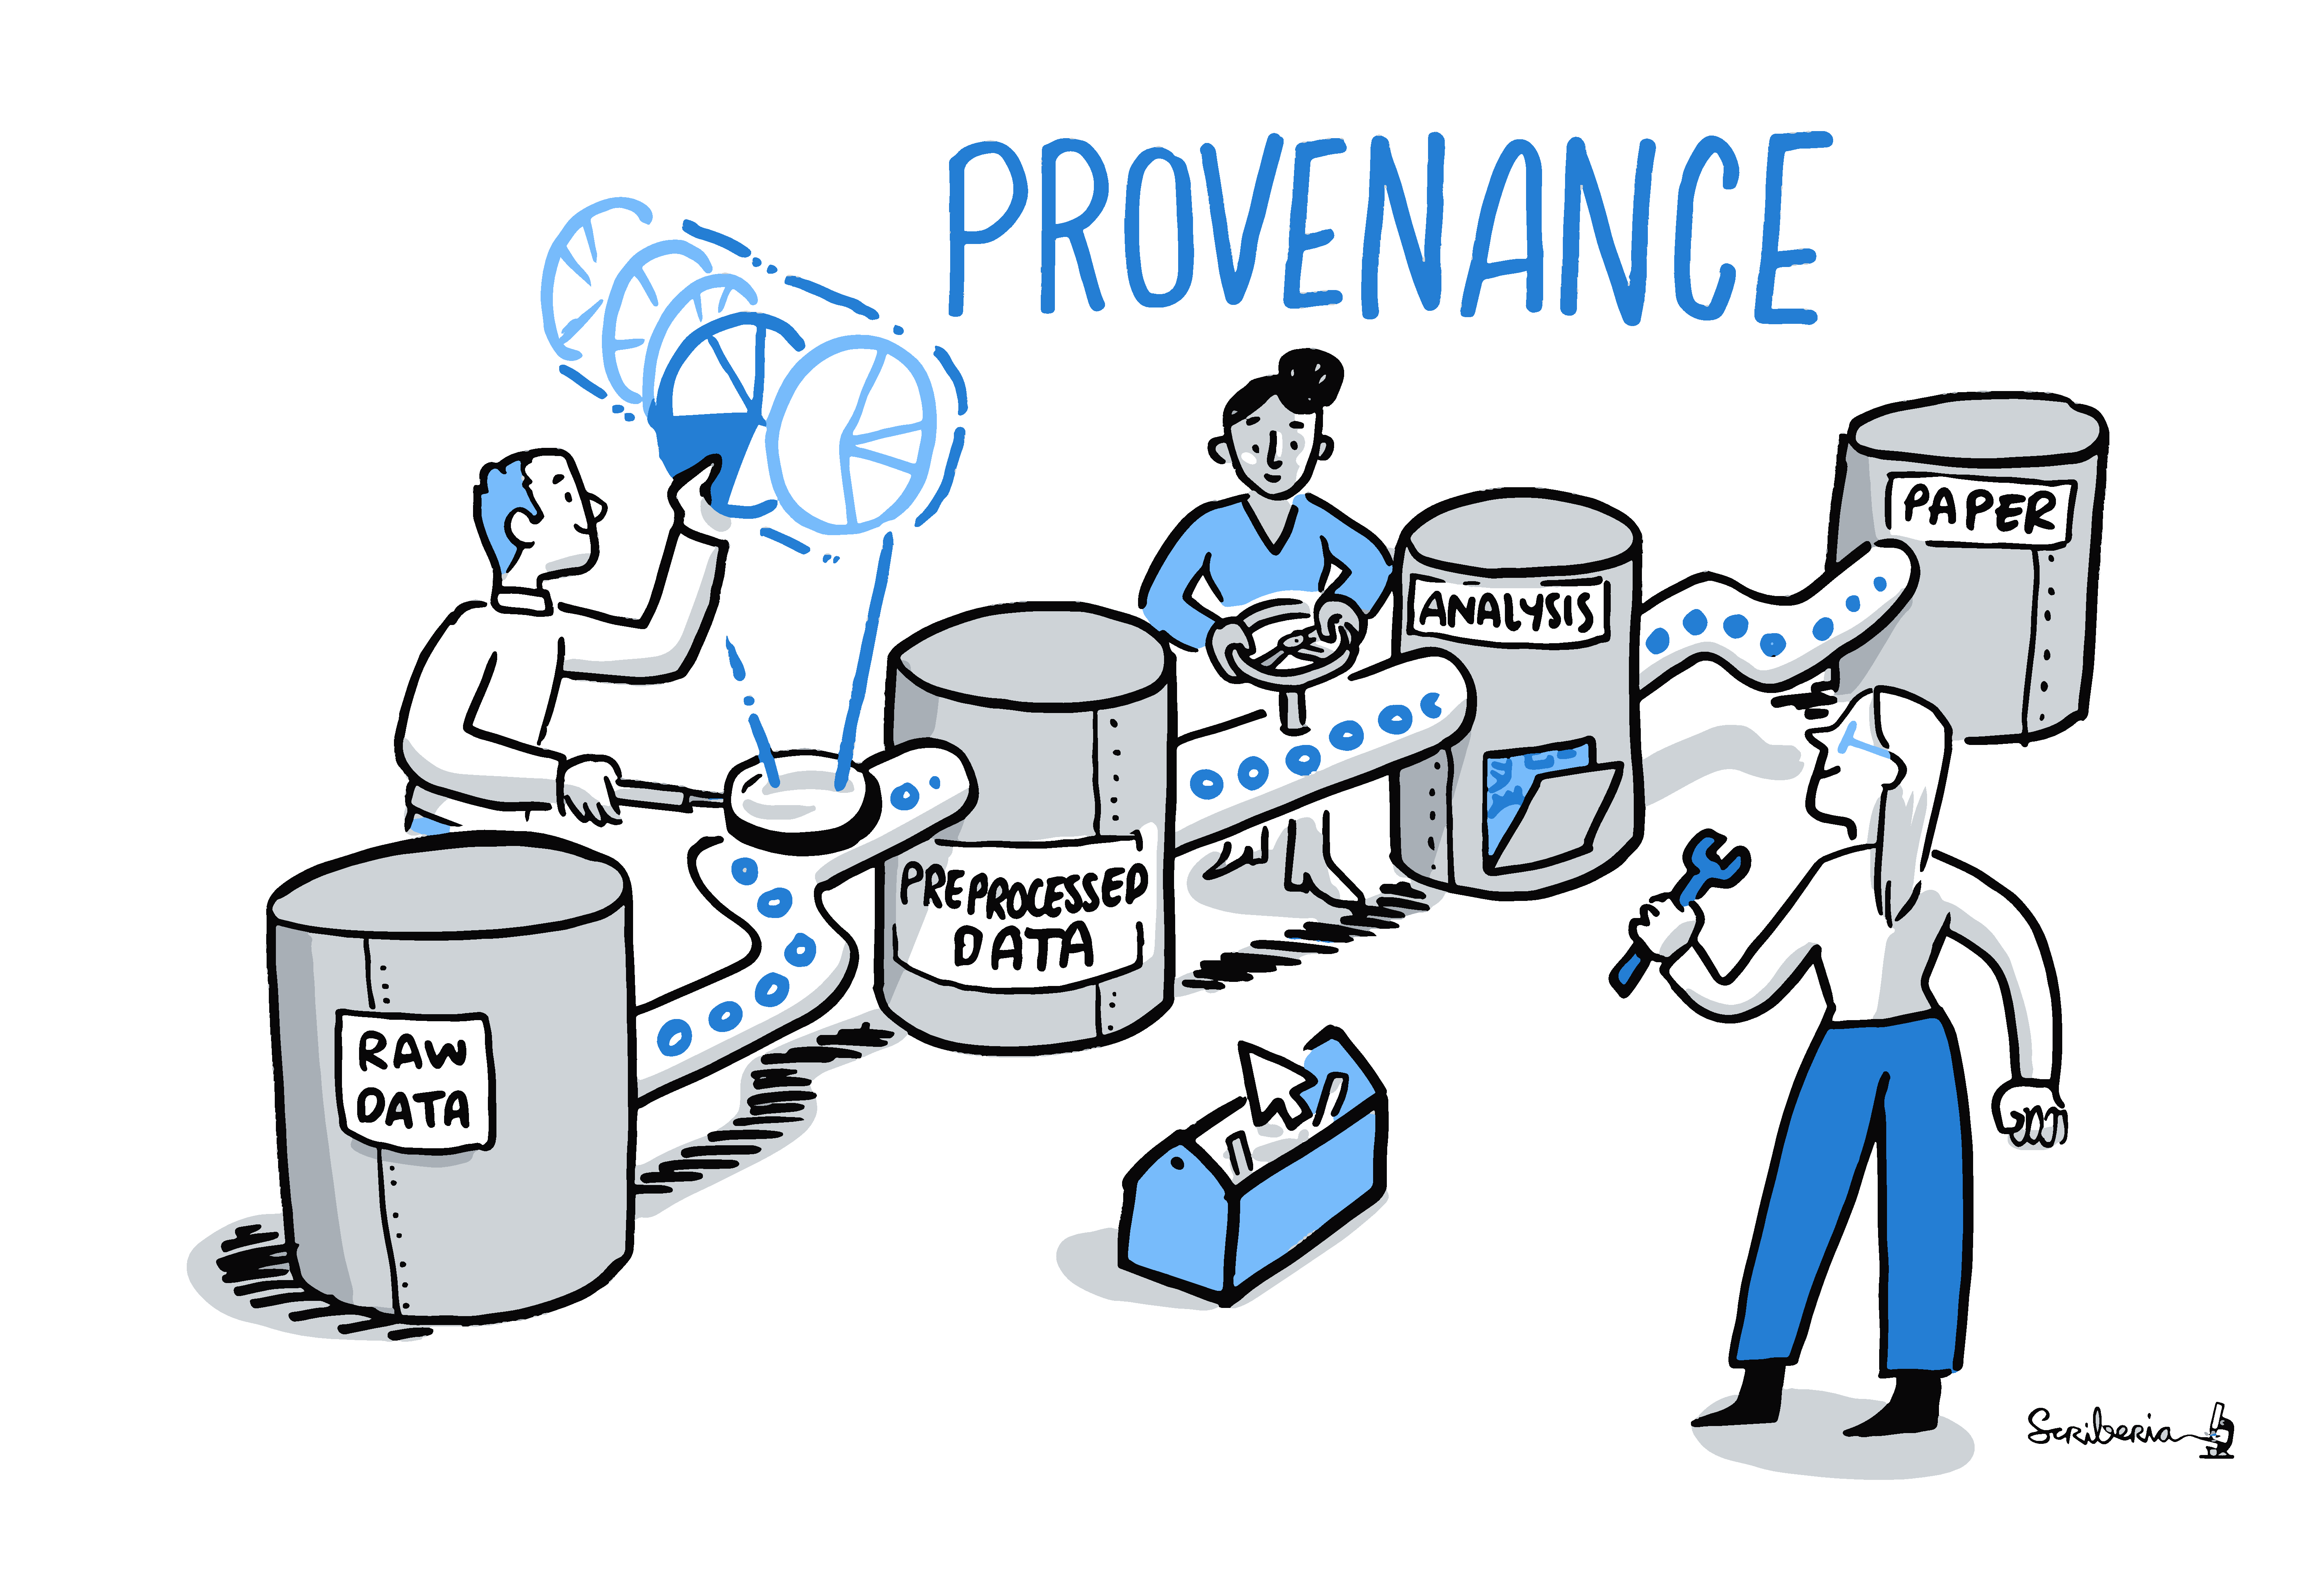
\includegraphics[width=\textwidth]{provenance.pdf}
	\caption{License: Scriberia and the Turing Way Project, CC-BY}
	\label{fig:prov1}
\end{figure}


% link to chapter 3: Research data management is a prerequisite of reproducible research

\pagebreak

\section{DataLad as a software solution for research data management challenges}

Parts of this section were published as \citet{Halchenko2021}: ``DataLad: distributed system for joint management of code, data, and their relationship'' and are appropriately marked as such.
%This introduces DataLad as a software solution for research data management

%% from datalad paper:

Code, data and computing environments are core components of scientific projects. While
the collaborative development and use of research software and code is streamlined with es-
tablished procedures and infrastructures, such as software distributions, distributed version
control systems, and social coding portals like GitHub, other components of scientific projects
are not as transparently managed or accessible. Data consumption is complicated by discon-
nected data portals that require a large variety of different data access and authentication
methods. Compared with code in software development, data tend not to be as precisely
identified because data versioning is rarely or only coarsely practiced. Scientific computation
is not reproducible enough, because data provenance, the information of how a digital file
came to be, is often incomplete and rarely automatically captured. Last but not least, in
the absence of standardized data packages, there is no uniform way to declare actionable
data dependencies and derivative relationships between inputs and outputs of a computa-
tion. DataLad aims to solve these issues by providing streamlined, transparent management
of code, data, computing environments, and their relationship. It provides targeted interfaces
and interoperability adapters to established scientific and commercial tools and services to
set up unobstructed, unified access to all elements of scientific projects. This unique set of
features enables workflows that are particularly suited for reproducible science, such as ac-
tionable process provenance capture for arbitrary command execution that affords automatic
re-execution. To this end, it builds on and extends two established tools for version control
and transport logistics, Git and git-annex.

\pagebreak

